%%%%%%%%%%%%%%%%%%%%%%%%%%%%%%%%%%%%%%%%%%%%%%%%%%%%%%%%%%%%%%%%%%%%%%%%%%%%%%%%%%%%%%%%%%%%%%%%%%%%%%%
%%%%%%%%%%%%%% Template de Artigo Adaptado para Trabalho de Diplomação do ICEI %%%%%%%%%%%%%%%%%%%%%%%%
%% codificação UTF-8 - Abntex - Latex -  							     %%
%% Autor:    Fábio Leandro Rodrigues Cordeiro  (fabioleandro@pucminas.br)                            %% 
%% Co-autores: Prof. João Paulo Domingos Silva, Harison da Silva e Anderson Carvalho		     %%
%% Revisores normas NBR (Padrão PUC Minas): Helenice Rego Cunha e Prof. Theldo Cruz                  %%
%% Versão: 1.1     18 de dezembro 2015                                                               %%
%%%%%%%%%%%%%%%%%%%%%%%%%%%%%%%%%%%%%%%%%%%%%%%%%%%%%%%%%%%%%%%%%%%%%%%%%%%%%%%%%%%%%%%%%%%%%%%%%%%%%%%
\section{Introdução}
O problema do caixeiro viajante é um desafio clássico na área de otimização combinatória e tem sido extensivamente estudado e pesquisado ao  longo de décadas. Consiste em determinar a rota mais curta que um caixeiro precisa percorrer para visitar um conjunto de cidades uma única vez e, em seguida, retornar à cidade de origem. Neste trabalho, iremos realizar uma análise comparativa entre dois métodos amplamente utilizados para resolver o problema do caixeiro viajante: Branch and Bound e Força Bruta.

\section{Problema Proposto}
Dentre um conjunto de lojas, devemos buscar e levar produtos entre elas com o menor gasto de combustível possível. Cada produto que colocamos no caminhão diminui o rendimento do caminhão em 0.5 km/litro, sendo o rendimento quando vazio 10 km/litro. Esse problema é bem parecido com o problema do caixeiro viajante - um dos desafios mais conhecidos e estudados na área de otimização combinatória, que consiste em encontrar a rota mais curta possível que um caixeiro precisa percorrer para visitar um conjunto de cidades uma única vez e retornar à cidade de origem

\section{Solução proposta}
Nosso objetivo é analisar e estudar o método Branch and Bound, comparando seus resultados com o método de Força Bruta. Ambos os métodos são utilizados para solucionar o problema do caixeiro viajante, mas diferem em termos de eficiência e desempenho.

O método de Força Bruta consiste em testar todas as possíveis combinações de rotas para encontrar a solução ótima, o que pode ser extremamente custoso computacionalmente, especialmente quando o número de cidades é grande. Por outro lado, o método Branch and Bound é uma técnica que busca evitar a exploração de todas as combinações possíveis, utilizando limites superiores e inferiores para podar ramos da árvore de busca e reduzir o espaço de soluções a ser explorado.

No algoritmo baseado em Força Bruta, geramos uma lista com todos os caminhos válidos, e depois pegamos o com o menor custo. Já no baseado em Branch and Bound, temos um lower bound com uma heurística de custo e podamos caminhos que tem a heurística maior que o lower bound.

\section{Implementação}
A linguagem de programação Python foi escolhida para a codificação dos algoritmos, devido à sua facilidade de implementação e à disponibilidade de várias bibliotecas que auxiliam na visualização gráfica da solução encontrada pelo algoritmo. Os algoritmos de Força Bruta e Branch and Bound possuem estruturas similares, com classes e métodos semelhantes.

O algoritmo de Força Bruta é mais simples de ser implementado e compreendido, pois envolve uma análise de todas as possibilidades, mesmo as infrutíferas. Isso significa que o algoritmo examina todas as combinações possíveis de soluções, o que pode ser ineficiente em termos de tempo de execução, especialmente para problemas com um grande número de soluções possíveis.

Por outro lado, o algoritmo Branch and Bound possui um limite inferior de custo que serve como critério de poda para o problema, que armazena a melhor solução encontrada até o momento. Com base nesse valor, caminhos que não levarão a uma solução melhor são descartados, o que pode melhorar significativamente o desempenho do algoritmo. Em seu pior caso, não conseguiremos realizar nenhuma poda, o que é equivalente à complexidade do algoritmo de Força Bruta, pois todos os caminhos possíveis seriam checados.

\section{Relatório de testes}
Para analisar o tempo de execução exponencial dos dois algoritmos, foram realizados experimentos em cinco cenários diferentes, nos quais o número de elementos aumentou proporcionalmente. Essa análise é uma forma simples de entender o desempenho relativo do método Branch and Bound em comparação à abordagem de Força Bruta.

\subsection{Primeiro Cenário}
No primeiro cenário, considerou-se um problema de tamanho pequeno, com um número limitado de elementos. Nesse caso, a diferença de desempenho entre os dois algoritmos não foi muito significante, já que ambos encontraram a solução ótima com a mesma quantidade de iterações. 

\newpage

Rodamos ambos os algoritmos com o seguinte conjunto de 6 lojas:
\begin{figure}[!ht]
	\centering	
	\caption[\hspace{0.1cm}Cenário 1]{Cenário 1}
	  \vspace{-0.4cm}
	\includegraphics[width=.3\textwidth]{figuras/cenário1.png}
\end{figure}

E obtivemos os seguintes resultados:

Branch And Bound: 0.0079 segundos, 60 iterações

Força Bruta: 0.0149 segundos, 60 iterações

\subsection{Segundo Cenário}
No segundo cenário, o tamanho do problema foi aumentado para um número moderado de elementos. Nesse estágio, a abordagem de força bruta começa a mostrar sinais de ineficiência, uma vez que precisa examinar todas as possíveis soluções. 

Rodamos ambos os algoritmos com o seguinte conjunto de 10 lojas:
\begin{figure}[!ht]
	\centering	
	\caption[\hspace{0.1cm}Cenário 2]{Cenário 2}
	  \vspace{-0.4cm}
	\includegraphics[width=.3\textwidth]{figuras/cenário2.png}
\end{figure}

E obtivemos os seguintes resultados:

Branch And Bound: 0.7207 segundos, 15993 iterações

Força Bruta: 9.8962 segundos, 36517 iterações

\subsection{Terceiro Cenário}
No terceiro cenário, com um número ainda maior de elementos, a diferença de desempenho entre os dois algoritmos se torna bem mais evidente. Por outro lado, o método Branch and Bound continua a se beneficiar de sua estratégia de busca inteligente. 

Rodamos ambos os algoritmos com o seguinte conjunto de 14 lojas:
\begin{figure}[!ht]
	\centering	
	\caption[\hspace{0.1cm}Cenário 3]{Cenário 3}
	  \vspace{-0.4cm}
	\includegraphics[width=.3\textwidth]{figuras/cenário3.png}
\end{figure}

E obtivemos os seguintes resultados:

Branch And Bound: 1.7875 segundos, 60068 iterações

Força Bruta: 69.6516 segundos, 254779 iterações

\section{Conclusão}
Conclui-se então, que o método Branch and Bound é uma alternativa superior ao de Força Bruta, já que em seu pior caso irá apresentar o mesmo número de iterações que o caso médio de Força Bruta, por ser uma melhoria direta à ele.

A priori, Branch and Bound permite uma busca mais inteligente e eficiente ao dividir o espaço de busca em regiões menores e mais gerenciáveis. Isso reduz significativamente o número de soluções a serem consideradas, o que é especialmente benéfico em problemas de otimização com espaços de busca extensos. Ao contrário da abordagem de força bruta, que examina todas as possíveis soluções, o Branch and Bound é capaz de descartar regiões inteiras do espaço de busca que não têm potencial para fornecer uma solução ótima, economizando tempo.

A posteriori, o método Branch and Bound utiliza limites inferiores para avaliar e comparar soluções parciais. Essa técnica permite a poda de ramos da árvore de busca que não têm potencial para fornecer uma solução melhor do que a já encontrada. Como resultado, o método é capaz de reduzir ainda mais o número de soluções a serem avaliadas, aumentando a eficiência geral do algoritmo.

Mediante a isso e aos dados apresentados, concluímos que o uso do método Branch and Bound nesse problema oferece várias vantagens em relação à abordagem de Força Bruta.

\section{Participação}
Todos os integrantes do grupo participaram ativamente de todas as etapas do projeto, incluindo a confecção do documento, a programação e a análise dos algoritmos. Com o objetivo de aumentar nossa eficiência durante a elaboração do projeto, utilizamos a ferramenta Live Share disponibilizada pelo VSCode. Essa ferramenta possibilitou que todos os membros pudessem editar o código simultaneamente, colaborando de forma mais efetiva e em tempo real.

\begin{figure}[!ht]
	\centering	
	\caption[\hspace{0.1cm}Cenário 3]{Cenário 3}
	  \vspace{-0.4cm}
	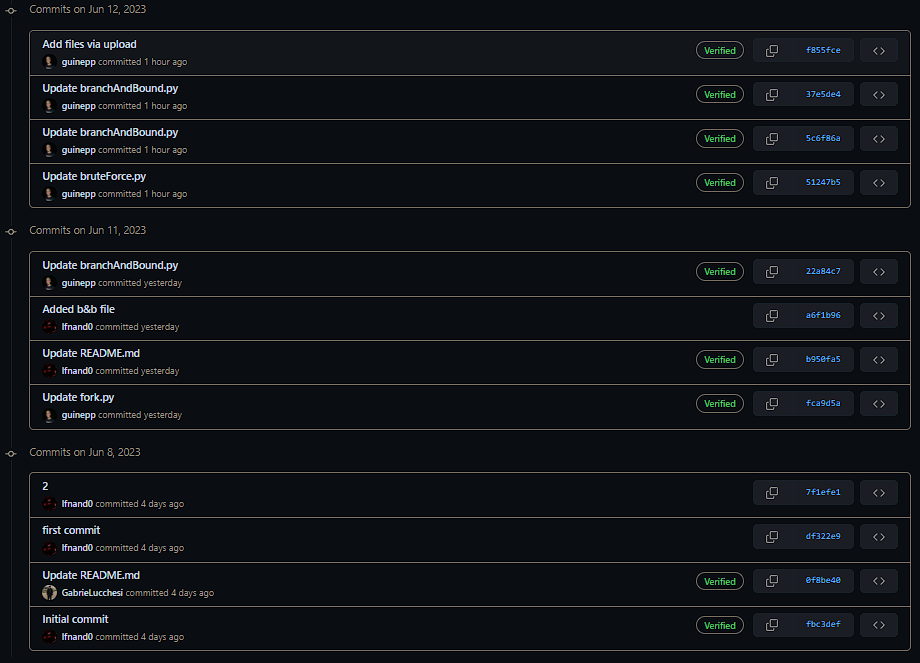
\includegraphics[width=.8\textwidth]{figuras/commits.png}
\end{figure}

\section{\esp REPOSITÓRIO}
Link do Repositório do trabalho: https://github.com/lfnand0/Trab2-PAA